\section[Radius Selection]{Phase 1: Radius Selection}

\begin{frame}[t]{Why DBSCAN?}{}
    \vspace{-0.3cm}
    \begin{columns}[T]
        \column{0.50\textwidth}
        \begin{block}{1. Native Noise Detection}
            \vspace{0.1cm}
            {\small K-Means and GMMs \textbf{force} every point into a cluster. DBSCAN explicitly flags isolated points as \texttt{noise} ($-1$), preventing rural outliers from distorting urban cluster geometry.}
            \vspace{0.1cm}
        \end{block}
        \vspace{0.2cm}
        \begin{block}{2. Arbitrary Density Manifolds}
            \vspace{0.1cm}
            {\small K-Means assumes \textbf{spherical} clusters with linear Voronoi boundaries. DBSCAN links points via contiguous density, capturing elongated urban corridors (e.g., Rhine-Ruhr) without imposing geometric priors.}
            \vspace{0.1cm}
        \end{block}

        \column{0.50\textwidth}
        \begin{block}{3. Physical Parameterization}
            \vspace{0.1cm}
            {\small DBSCAN replaces abstract $k$ with physically meaningful hyperparameters:}
            \begin{itemize}
                \setlength\itemsep{4pt}
                \item {\small $\varepsilon = 40\,\text{km}$ \;---\; max.\ tower signal range}
                \item {\small $\text{min\_samples} = 2$ \;---\; urban density threshold}
            \end{itemize}
            \vspace{0.1cm}
            {\small Distance metric: \textbf{haversine} (great-circle), which accounts for Earth's curvature when converting lat/lon to true ground distances.}
            \vspace{0.1cm}
        \end{block}
    \end{columns}
\end{frame}

\begin{frame}[t]{Spatial Clustering (DBSCAN)}{}
    \begin{columns}[T]
        % 1. Left Column: The cluster map
        \column{0.60\textwidth}
        \begin{center}
            \vspace{-1.3cm} 
            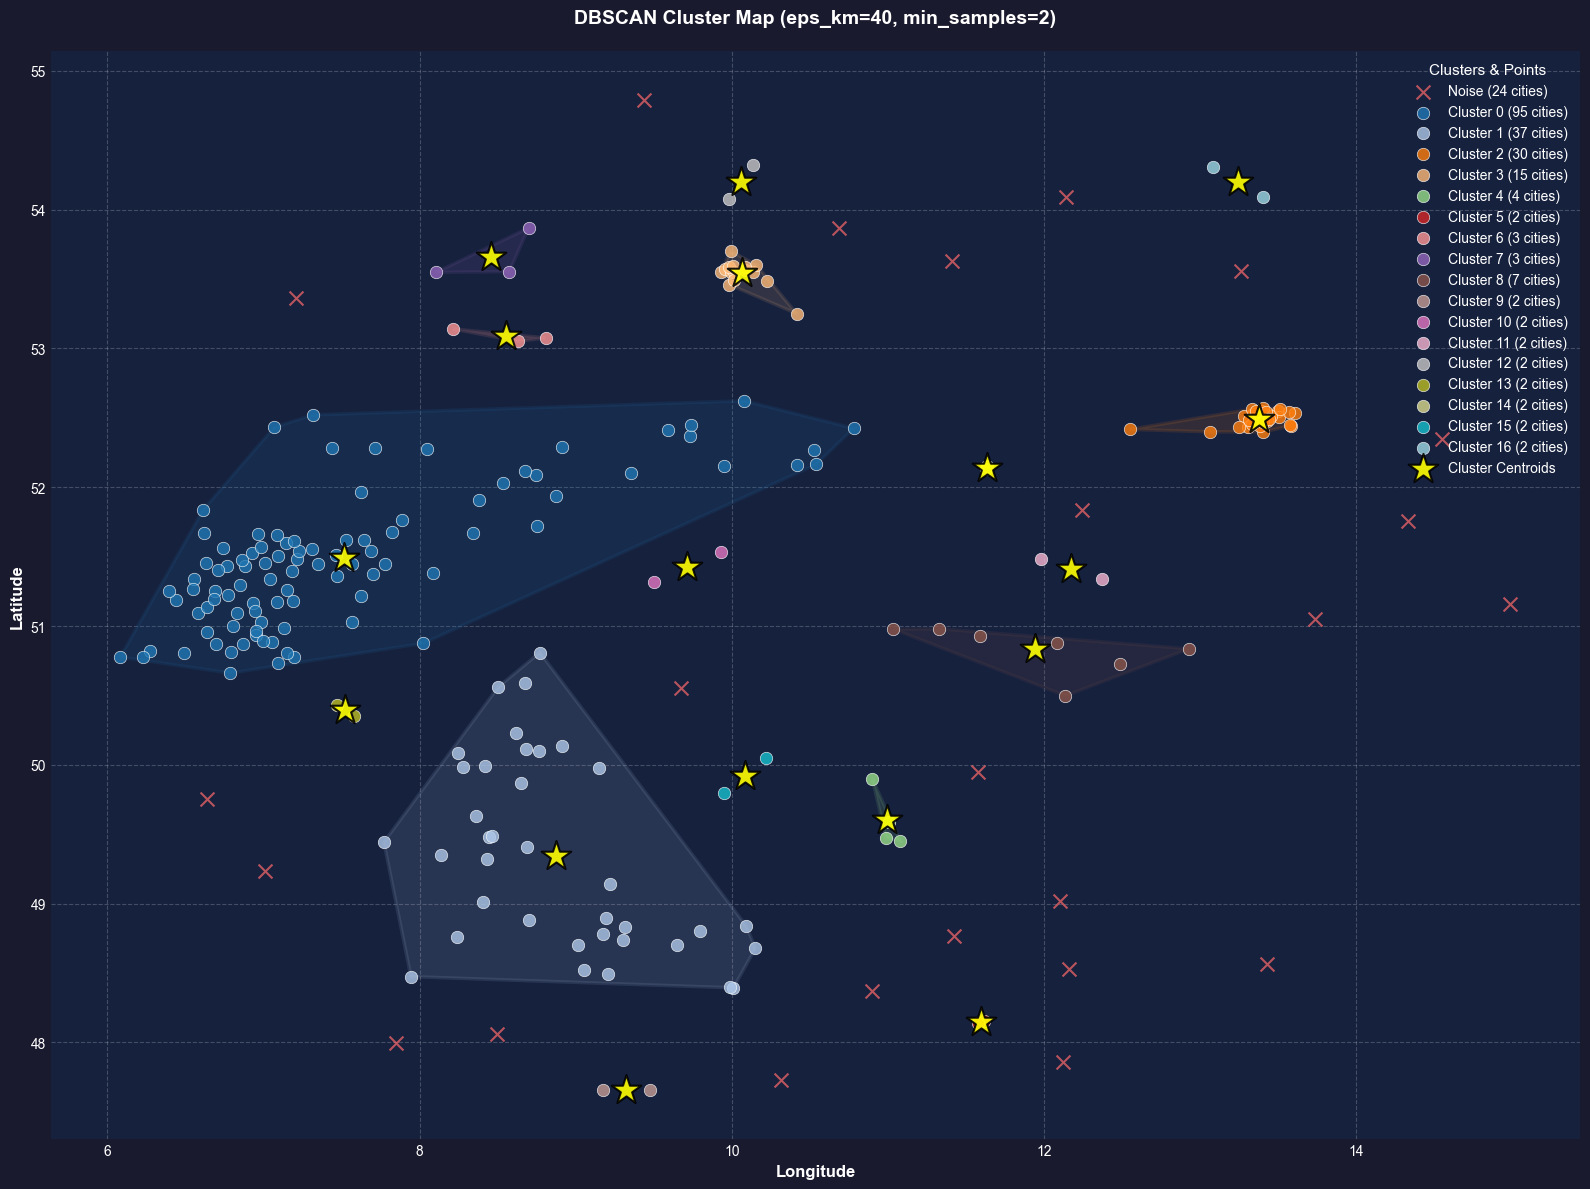
\includegraphics[width=\textwidth,height=0.80\textheight,keepaspectratio]{./images/clusters.png}
        \end{center}

        % 2. NEW Middle Column: Acts as your X-axis slider!
        \column{-1.0\textwidth}

        % This column stays completely empty to push the box to the right.
        % Increase 0.06 to push the box further right; decrease it to pull it left.
        % 3. Right Column: Contains the hyperparameter block
        \column{0.24\textwidth}
        \vspace{1.0cm} 

        \begin{block}{\centering Parameter}
            \centering
            \vspace{0.1cm}
            {\small $\varepsilon = 40\,\text{km}$} \\[4pt]
            {\small $\text{min\_samples} = 2$}
            \vspace{0.1cm}
        \end{block}
    \end{columns}
\end{frame}


\begin{frame}[t]{Computing Radius Search Bounds}{}
    \begin{center}
    \begin{minipage}{0.92\textwidth}
        \textbf{Why bounds?}\\[4pt]
        Searching all of $[5,100]$\,km is mathematically wasteful and computationally inefficient. The geographic data inherently dictates our optimal search horizon.
    \end{minipage}
    \end{center}
    \vspace{0.4cm}
    \begin{columns}[T]
        % Left Box: Lower Bound Mathematics
        \column{0.48\textwidth}
        
        \vspace{-0.45cm} % adjust to align with right block
        
        \begin{center}
        \begin{minipage}{0.92\textwidth}
            \begin{block}{Lower Bound ($r_{\min}$)}
                \begin{equation*}
                    r_{\min} = \max\!\Big(5,\; \big\lfloor \tfrac{P_{10}(\text{NN})}{2} \big\rfloor\Big)
                \end{equation*}
                \vspace{0.1cm}
                {\small Sets threshold using half the 10\textsuperscript{th} percentile of nearest-neighbor distances. Prevents over-allocating tiny towers in high-density zones.}
            \end{block}
        \end{minipage}
        \end{center}

        % Right Box: Upper Bound Mathematics
        \column{0.48\textwidth}
        \vspace{-0.45cm} % move up/down
        \begin{center}
        \begin{minipage}{0.92\textwidth} % adjust width here
            \begin{block}{Upper Bound ($r_{\max}$)}
                \begin{equation*}
                    r_{\max} = \min\!\Big(100,\; \big\lceil P_{95}(\text{pairwise}) \big\rceil\Big)
                \end{equation*}
                \vspace{0.1cm}
                {\small Sets threshold using the 95\textsuperscript{th} percentile of all global pairwise distances. Caps wasteful spatial allocation.}
            \end{block}
        \end{minipage}
        \end{center}
    \end{columns}

\end{frame}
\begin{frame}[t]{Radius Search Bounds Plot}{}
    \begin{columns}[T]
        % Dominates the left with the layout plot
        \column{0.96\textwidth}
        \begin{center}
            \vspace{-1.3cm}             
\includegraphics[width=\textwidth,height=0.80\textheight,keepaspectratio]{./images/radius_bounds_visual.png}
        \end{center}
        % Spacer column to slide box cleanly along the X-axis
        \column{0.04\textwidth}
    \end{columns}
\end{frame} 

% ==========================================
% SLIDE 4: RADIUS OPTIMIZATION METHODOLOGY
% ==========================================
\begin{frame}[t]{Coarse to Fine Radius Search}{}
    \vspace{0.2cm}
    \begin{columns}[T]
        
        % Left Column: The Mathematical Objective
        \column{0.35\textwidth}
        \begin{block}{1. Scoring Function} 
            \vspace{0.2cm}
            \begin{equation*}
                 J(r) = \frac{\overbrace{\text{cost}(r)}^{\text{installation cost}}}{\underbrace{\max\big(1,\; \overline{\text{cov}}(r)\big)}_{\text{avg.\ cities covered}}}  
            \end{equation*}
            \vspace{0.3cm}                                                    
        \end{block}

        % Right Column: The Search Strategy
        \column{0.48\textwidth}
        \begin{block}{2. Coarse-to-Fine}
            \begin{center}
                \begin{tikzpicture}[scale=0.85, >=stealth]
                    % Draw axes
                    \draw[->, gray, thick] (0,0) -- (6.5,0) node[right, font=\footnotesize] {Radius};
                    \draw[->, gray, thick] (0,0) -- (0,3.0) node[above, font=\footnotesize] {Score};

                    % Draw "Cost Landscape" curve
                    \draw[FAUBlue, very thick] plot[smooth, tension=0.7] coordinates {
                        (0.5, 2.6) (1.8, 1.2) (3.2, 1.9) (4.5, 0.4) (5.8, 2.3)
                    };

                    % Coarse Search (Big jumps)
                    \draw[<->, gray, dashed] (0.5, -0.3) -- (1.8, -0.3) node[midway, below, font=\tiny] {15km step};
                    \fill[red!80] (0.5, 2.6) circle (2.5pt);
                    \fill[red!80] (1.8, 1.2) circle (2.5pt);
                    \fill[red!80] (3.2, 1.9) circle (2.5pt);
                    \fill[red!80] (4.5, 0.4) circle (2.5pt);
                    \fill[red!80] (5.8, 2.3) circle (2.5pt);

                    % Fine Search (Zoom box)
                    \draw[FAUGreen, thick, rounded corners, dashed] (3.8, 0.1) rectangle (5.2, 1.1);
                    
                    % Little fine points around the global minimum
                    \fill[FAUGreen] (4.1, 0.7) circle (1.5pt);
                    \fill[FAUGreen] (4.3, 0.5) circle (1.5pt);
                    \fill[FAUGreen] (4.5, 0.4) circle (1.5pt);
                    \fill[FAUGreen] (4.7, 0.6) circle (1.5pt);
                    \fill[FAUGreen] (4.9, 0.9) circle (1.5pt);
                    
                    % Global Min star
                    \node[text=orange, font=\large] at (4.5, 0.4) {$\bigstar$};
                \end{tikzpicture}
            \end{center}
            
            \vspace{0.1cm}
            {\footnotesize
            \textbf{Step 1 (Coarse):} Test large 15\,km intervals (red dots) to rapidly locate the general performance "valley."\\[4pt]
            \textbf{Step 2 (Fine):} Zoom in on the top coarse result and test integer 1\,km steps within a $\pm 14$\,km window (green dots) to lock in the true global minimum ($\bigstar$).
            }
        \end{block}

    \end{columns}
\end{frame}

% ==========================================
% SLIDE 5: RADIUS OPTIMIZATION SCORES
% ==========================================
\begin{frame}[t]{Radius Optimization Scores}{}
    \begin{center}
        \vspace{0.2cm}
        
\includegraphics[width=0.95\textwidth,height=0.7\textheight,keepaspectratio]{./images/coarse_fine_score.png}
    \end{center}
\end{frame}
